\subsection{Schallgeschwindigkeitsbestimmung mit Echo-Impuls Verfahren}\label{sec:echo-impuls}
In diesem Experiment stehen vier Zylinder unterschiedlicher Höhe zur Verfügung, die mit Hilfe der Ultraschallsonde vermessen werden. Zunächst wird die Höhe mit einer Schieblehre bestimmt (siehe Tabelle \ref{tab:zylinder}).

 \begin{figure}[h!]
 	\centering
 	\captionof{table}{Höhe der im Experiment verwendeten Zylinder}
 	\begin{tabular}{c|c}
 	Zylinder & Höhe in mm\\
 		\hline
  1 & 31.10 \\
  2 & 61.50 \\
  3 & 80.45 \\
  4 & 120.75 \\
 	\end{tabular}
 	\label{tab:zylinder}
 \end{figure}
 
 Mit diesen Zylindern und zwei Kombinationen aus ihnen wird eine Laufzeitmessung durchgeführt. Das Signal für den kleinsten Zylinder ist in Abbildung \ref{fig:reflexion1} zu sehen. Aus der gemessenen Höhe $s $ und der Laufzeit $t$ kann die Schallgeschwindigkeit $c$ im Medium -- Acryl bestimmt werden. Problematisch ist die Grenzfläche und das Kontaktmittel zwischen Sonde und Zylinder. Eine lineare Ausgleichsrechnung aller Messdaten (siehe Tabelle \ref{tab:echo-impuls}) mit Hilfe von Python liefert einen genaueren Wert für $c$ und zusätzlich die Dicke $b$ der Anpassungsschicht. Der Plot ist in Abbildung \ref{fig:regression1} dargestellt. 
 \begin{align}
 	s = \frac{1}{2} \, c \, t + b
 \end{align}
 
 \begin{align}
 	c = \input{build/v_Echo-Impuls.txt} \\
 	b = \input{build/b_Echo-Impuls.txt}
 \end{align}

 \begin{figure}[h!]
 	\centering
 	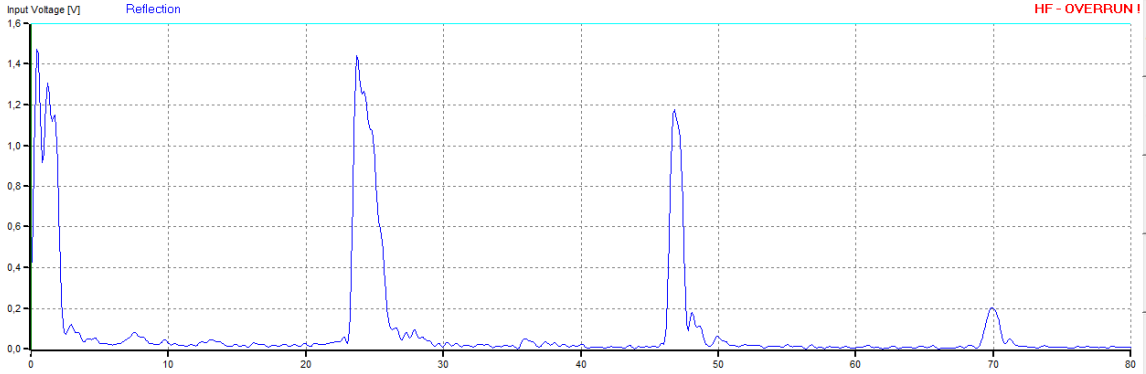
\includegraphics[width=\textwidth]{Messung_1.png}
 	\caption{Reflexion am Zylinder (\SI{33.1}{\milli\meter})}
 	\label{fig:reflexion1}
 \end{figure}


 \begin{figure}[h!]
 	\centering
 	\captionof{table}{Laufzeiten des Echo-Impuls Verfahren}
 	\begin{tabular}{c|c}
 		Laufzeit in $s^{-5}$ & Zylinderhöhe in mm\\
 		\hline
 		\input{build/tabelle_echo-impuls.txt}
 	\end{tabular}
 	\label{tab:echo-impuls}
 \end{figure}
 
 \begin{figure}[h!]
 	\centering
 	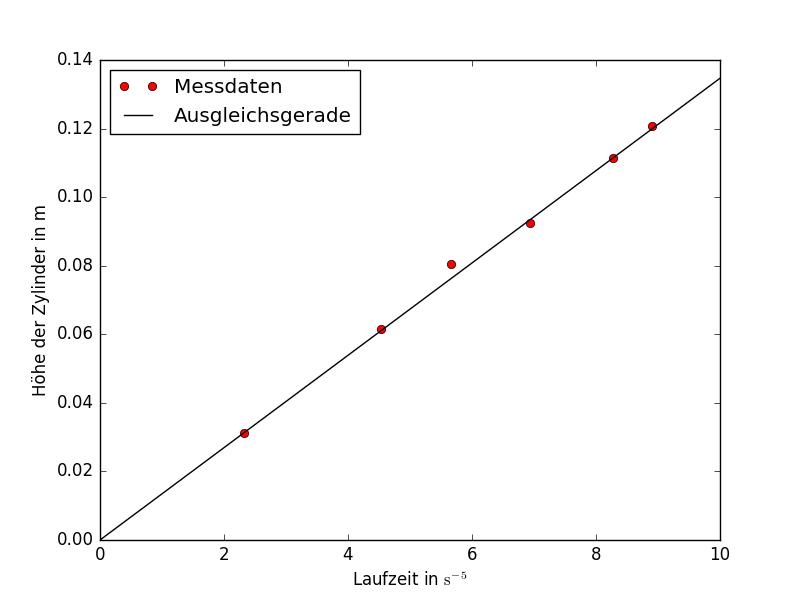
\includegraphics[width=0.7\textwidth]{build/Impuls-Echo.png}
 	\caption{Laufzeiten des Echo-Impuls Verfahrens über die Höhe der Zylinder aufgetragen}
 	\label{fig:regression1}
 \end{figure}
 

 
 
 
 \clearpage
 \subsection{Schallgeschwindigkeitsbestimmung mit Durchschallungs-Verfahren}
 Bei dem Durchschallungs-Verfahren wird die selbe Rechnung wie in Kapitel \ref{sec:echo-impuls} durchgeführt. Es muss allerdings berücksichtig werden, dass das Ultraschallsignal nur einmal durch den Körper geht
 \begin{align}
 	s =  c \, t + b
 \end{align}
 Hier ist lediglich ein anderer Wert für die Anpassungsschicht zu erwarten, da auf beiden Seiten Grenzflächen liegen. Die Daten der Regression sind in Tabelle \ref{tab:durchschall} und der Plot in Abbildung \ref{fig:durchschall} dargestellt. Das Ergebnis ist
  \begin{align}
  	c = \input{build/v_Durchschall.txt} \quad ,\\
  	b = \input{build/b_Durchschall.txt} \quad .
  \end{align}
  
 
 \begin{figure}[h!]
 	\centering
 	\captionof{table}{Laufzeiten des Durchschall-Verfahren}
 	\begin{tabular}{c|c}
 		Laufzeit in $s^{-5}$ & Zylinderhöhe in mm\\
 		\hline
 		\input{build/tabelle_Durchschall.txt}
 	\end{tabular}
 	\label{tab:durchschall}
 \end{figure}
 
 \begin{figure}[h!]
 	\centering
 	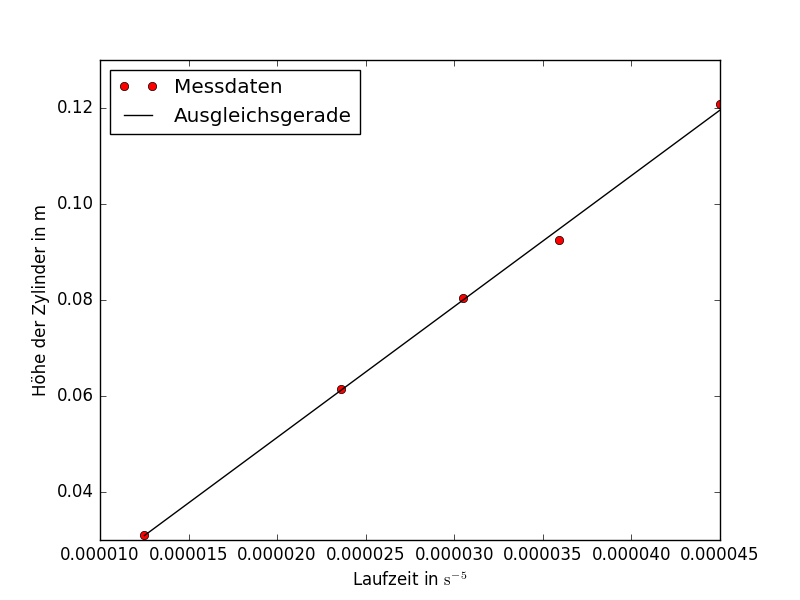
\includegraphics[width=0.7\textwidth]{build/Durchschall.png}
 	\caption{Laufzeiten des Durchschall-Verfahrens über die Höhe der Zylinder aufgetragen}
 	\label{fig:durchschall}
 \end{figure}
 


  
  
  \clearpage
  \subsection{Dickebestimmung der Acrylplatten} 
  Zur Bestimmung der Dicke zweier aufeinander liegender Acrylplatten wird das Impuls-Echo Verfahren verwendet und zusätzlich der kleine Zylinder zwischen Sonde und Platten angeordnet. Die Schallgeschwindigkeit in Acryl ist aus den vorherigen Kapiteln bekannt. für eine höhere Genauigkeit soll hier der Mittelwert verwendet werden
  \begin{align}
  	c = \frac{c_1+ c_2}{2} = \input{build/v_mittel.txt} \quad .
  \end{align}
  Die Laufzeitdifferenzen können hier besser im Cepstrum (siehe Abbildung~\ref{fig:cepstrum}) als im Originalbild abgelesen werden. Sie sind in Tabelle \ref{tab:laufzeiten_platte} dargestellt.
  
   \begin{figure}[h!]
   	\centering
   	\captionof{table}{Laufzeiten zur Berechnung der Dicke der Acrylplatten}
   	\begin{tabular}{c|c}
   	 & Laufzeit in \si{\micro\second}\\
   		\hline
   	1. Maximum & 13.5 \\
   	2. Maximum & 22.74 \\
   	3. Maximum & 35.7 \\
   	\end{tabular}
   	\label{tab:laufzeiten_platte}
   \end{figure}
  
  
   \begin{figure}[h!]
  	\centering
  	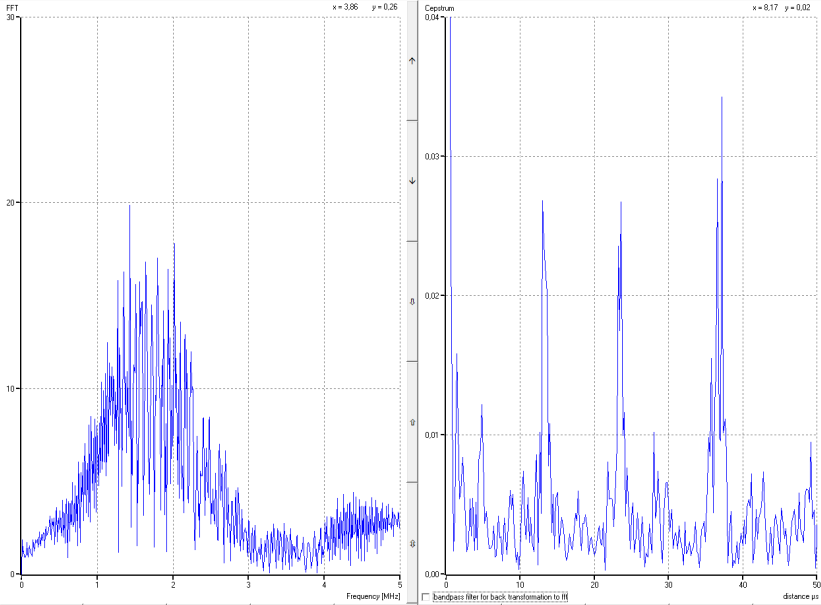
\includegraphics[width=\textwidth]{Messung_2.png}
  	\caption{Fast Fourier Tansformation und zugehöriges Cepstrum}
  	\label{fig:cepstrum}
  \end{figure}
  
  \clearpage
  
  Die Dicke der ersten Platte $h_1$ ergibt sich aus der Laufzeitdifferenz des ersten und zweiten Maximums und die Dicke der zweiten $h_2$  aus dem zweiten und dritten Maximum.
  \begin{align}
  	h_1 = \frac{1}{2} \,  c  \, (22.74 - 13.5)\si{\micro\second} = \SI{1.25 (2)}{\centi\meter} \\
  	  	h_2 = \frac{1}{2}\,  c \, (35.7 - 22.74)\si{\micro\second} = \SI{1.75(3)}{\centi\meter} 
  \end{align}
  
  
  
  
  
  
  
  
  \subsection{Abmessungen des Augenmodells}
Bei der Bestimmung der Maße des Augenmodels (siehe Abbildung \ref{fig:Auge}) mit Hilfe der Echo-Impuls Methode sind neben den Laufzeiten die unterschiedlichen Schallgeschwindigkeiten zu beachten:
\begin{align}
	& \text{Linse:} \quad c_\text{L} = \SI{2500}{\meter\per\second} \\
	& \text{Glaskörperflüssigkeit:} \quad c_\text{GK} = \SI{1410}{\meter\per\second} 
\end{align}
Die Laufzeiten in Abbildung \ref{fig:reflexion_auge} sind in Tabelle \ref{tab:laufzeiten_auge} zu finden.
Der Abstand von der Sonde zur Linse berechnet sich mit Hilfe des ersten Maximums
\begin{align}
	a_1 = \frac{1}{2}\cdot  c_\text{GK} \cdot \SI{11.6}{\micro\second} =
	\SI{8.2}{\milli\meter}  \quad .
\end{align}
Die Dicke der Linse ergibt sich auch der Laufzeitdifferenz des ersten und zweiten Maximums
\begin{align}
	a_2 = \frac{1}{2}\cdot  c_\text{L} \cdot (16.6-11.6)\si{\micro\second} =
	\SI{6.3}{\milli\meter}  \quad .
\end{align}
Um den Abstand von der Linse zur Retina zu berechnen werden das zweite und vierte Maximum verwendet. Das dritte Maximum entsteht aus der Doppelbrechung in der Linse und ist für die Rechnung irrelevant
\begin{align}
	a_3 = \frac{1}{2}\cdot  c_\text{L} \cdot (73.9-16.6)\si{\micro\second} =
	\SI{40.3}{\milli\meter}  \quad .
\end{align}
Das Auge hat somit im Gesamten eine Länge von 
\begin{align}
	a = a_1 + a_2 + a_3 = \SI{54.8}{\milli\meter} \quad .
\end{align}




	


   \begin{figure}[h!]
   	\centering
   	\captionof{table}{Laufzeiten zur Berechnung der Abmessungen des Auges}
   	\begin{tabular}{c|c}
   		& Laufzeit in \si{\micro\second}\\
   		\hline
   		1. Maximum & 11.6 \\
   		2. Maximum & 16.6 \\
   		3. Maximum & 23.5 \\
   		4. Maximum & 73.9
   	\end{tabular}
   	\label{tab:laufzeiten_auge}
   \end{figure}
  
  
  
  
  
    \begin{figure}[h!]
    	\centering
    	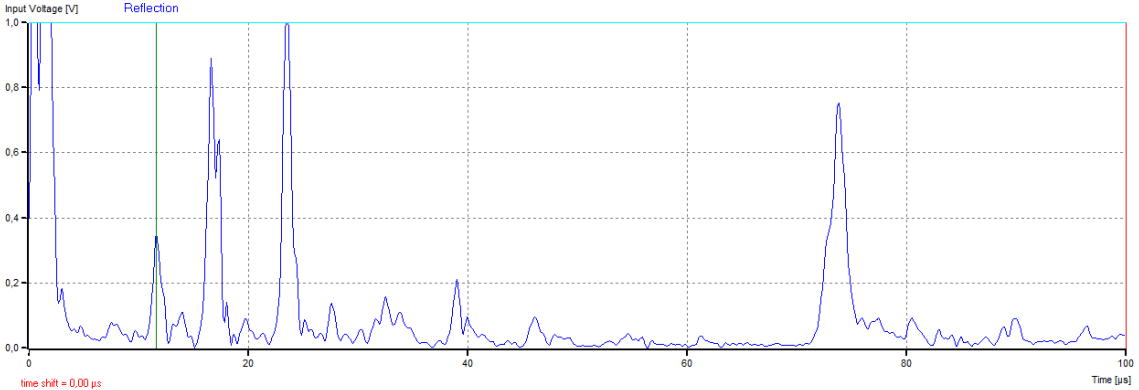
\includegraphics[width=\textwidth]{Messung_3.png}
    	\caption{Reflexionen am Augenmodell}
    	\label{fig:reflexion_auge}
    \end{figure}
  
 
 \todo[inline, color=red]{Annika fragen nach Achsensakllierung in Python}
 \todo[inline, color = red]{Wie ist das mit dem Seiten-Layout und den überschneidenden Überschriften?}
 